\documentclass[11pt,a4paper]{article}

\usepackage[utf8]{inputenc}
\usepackage[T1]{fontenc}
\usepackage{lmodern}
\usepackage[margin=2.5cm]{geometry}
\usepackage{graphicx}
\usepackage{float}
\usepackage{booktabs}
\usepackage{tabularx}
\usepackage{fancyhdr}
\usepackage[hidelinks]{hyperref}

\newcommand{\product}{AI Models Comparator}
\newcommand{\team}{Vivien GRUEL \\ Noé WALES \\ Valentin GEMPP \\ Maxence TESSIER}

\pagestyle{fancy}
\fancyhf{}
\fancyhead[L]{\product}
\fancyhead[R]{Software Design Description}
\fancyfoot[C]{\thepage}

\setlength{\emergencystretch}{3em}

\begin{document}

\begin{titlepage}
  \centering
  \vspace*{4cm}
  {\Huge\bfseries \MakeUppercase{\product}\par}
  \vspace{1.5cm}
  {\LARGE Software Design Description (SDD)\par}
  \vspace{4cm}
  {\large Software Engineering -- A4 -- 2026-2027\par}
  \vspace{1cm}
  {\large \team\par}
  \vfill
\end{titlepage}

\tableofcontents
\newpage

\section{Introduction}

\textbf{Purpose.} This document explains \textbf{how} the \product{} will be built. It describes the architecture, the data, the interfaces and the main technical choices, so that the developers can implement the system and the testers can check it.

\textbf{Scope.} The \product{} is a responsive web application. It shows AI models grouped by lab, a benchmark ranking, a community ranking based on up and down votes, a comment feed for each model, AI news, and an administration page.

\textbf{Audience.} Developers, testers and the TD instructor.

\textbf{References.} IEEE 1016-2009 (SDD), Business Requirements Document (BRD) and Software Requirements Specification (SRS) of the \product{}, SHMS SDD template given in the course.

\section{System Overview}

The \product{} is a classic three-tier web application:
\begin{itemize}
  \item a \textbf{frontend} in React with TypeScript (TSX components, built with Vite), which runs in the browser of the user;
  \item a \textbf{backend} in Node.js with Express, written in TypeScript, which contains the business logic and exposes a REST API;
  \item a \textbf{PostgreSQL database}, which stores all the data. The backend only accesses it through TypeORM: no SQL is written by hand.
\end{itemize}

The backend also runs scheduled jobs that import benchmark scores and AI news from external websites. The users never call these websites directly: they only read the data saved in our database. This way, the website still works when an external website is down.

\section{Architectural Views}

\subsection{Context View}

The system is between the human actors (visitors, registered users, administrators) and two kinds of external systems (benchmark source and news feed).

\begin{figure}[H]
  \centering
  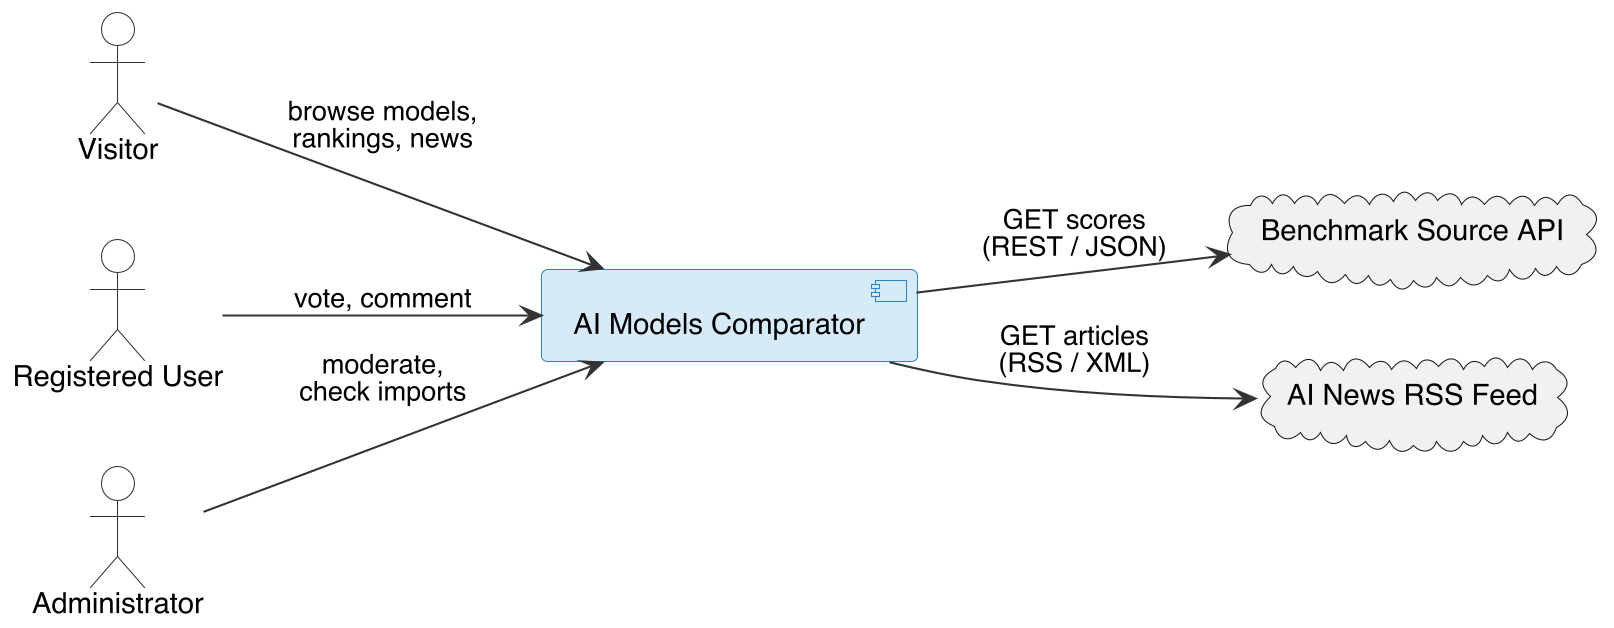
\includegraphics[width=0.9\textwidth]{figures/context.png}
  \caption{Context diagram}
\end{figure}

\textbf{Main interactions:}
\begin{itemize}
  \item \textbf{Visitors $\leftrightarrow$ system:} browse models, rankings and news, sign up, log in.
  \item \textbf{Registered users $\leftrightarrow$ system:} vote, comment, delete their comments and their account.
  \item \textbf{Administrators $\leftrightarrow$ system:} delete comments, block, unblock and delete users, check the imports.
  \item \textbf{System $\rightarrow$ benchmark source:} get the benchmark scores (REST, JSON).
  \item \textbf{System $\rightarrow$ news feed:} get the latest news (RSS, XML).
\end{itemize}

\subsection{Component View}

\begin{figure}[H]
  \centering
  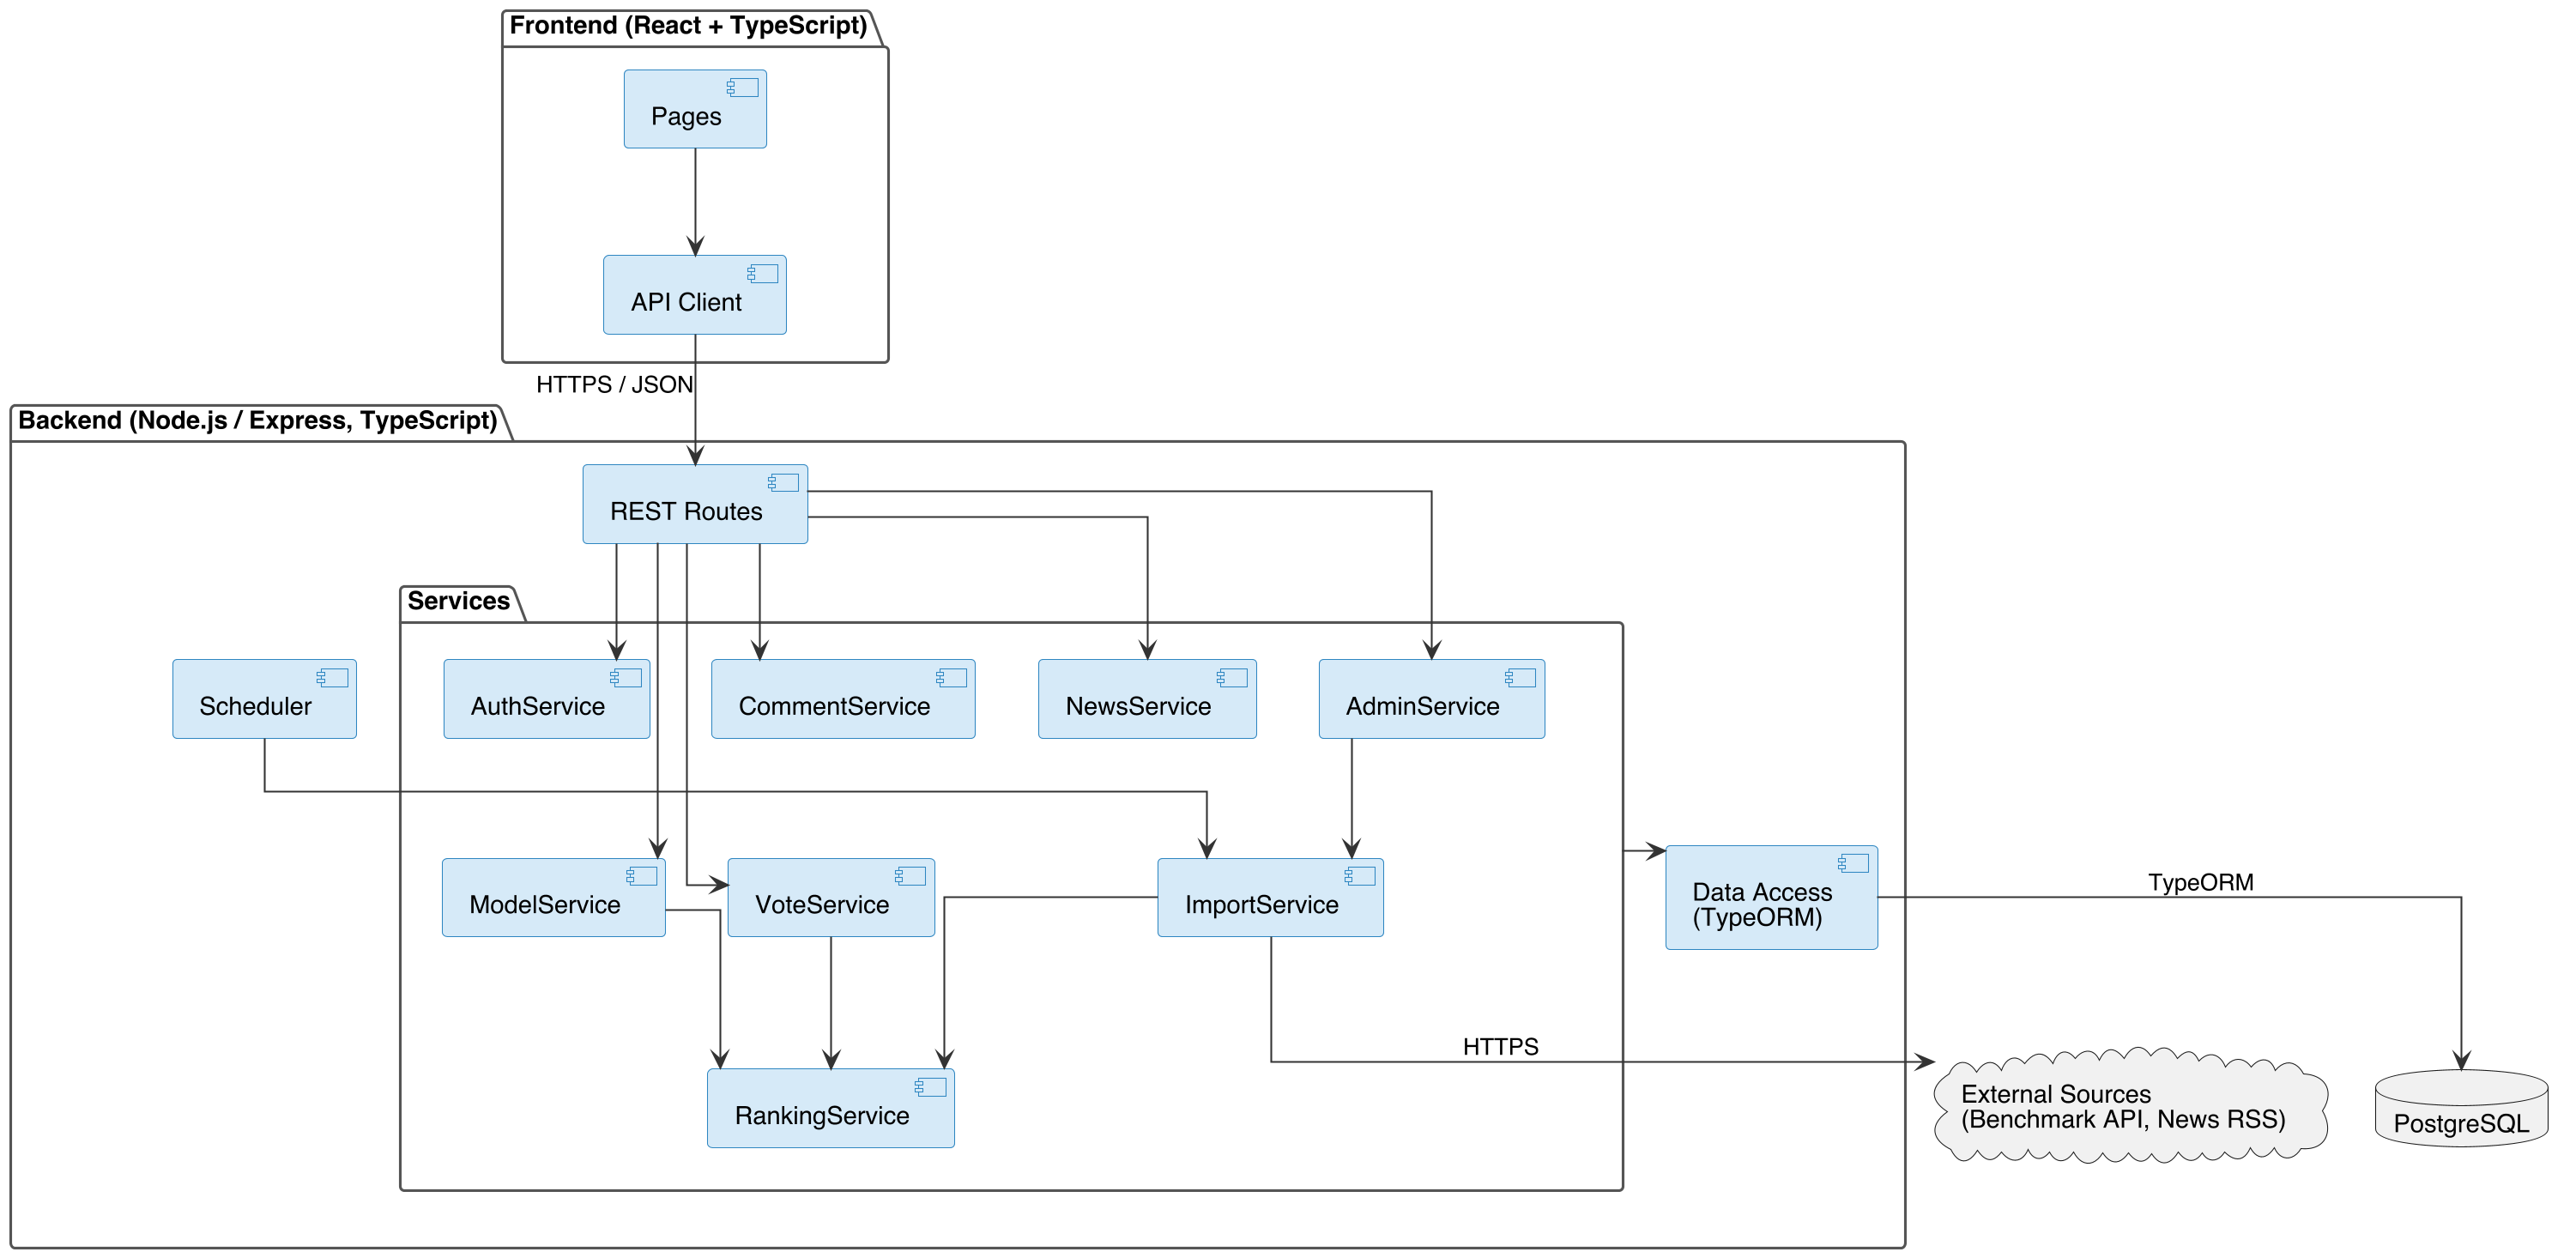
\includegraphics[width=\textwidth]{figures/components.png}
  \caption{Component diagram}
\end{figure}

\textbf{Components:}
\begin{itemize}
  \item \textbf{Pages} (frontend): one React component for each page of the SRS.
  \item \textbf{API Client} (frontend): sends the HTTP requests to the backend.
  \item \textbf{REST Routes}: receive the requests, check the session and the role, validate the inputs, and call the right service.
  \item \textbf{AuthService}: sign up, log in, log out, session management.
  \item \textbf{ModelService}: labs, models and model details (read from the database, with the stored scores and ranks).
  \item \textbf{VoteService}: add, change and remove votes.
  \item \textbf{CommentService}: add, list and delete comments.
  \item \textbf{RankingService}: computes the community and benchmark scores and the ranks, and saves them in the \texttt{models} table.
  \item \textbf{NewsService}: lists the news.
  \item \textbf{AdminService}: moderation of comments and users, import status, link of unknown model names.
  \item \textbf{ImportService}: downloads, checks and saves the data from the external sources.
  \item \textbf{Scheduler}: starts the imports at fixed times (node-cron).
  \item \textbf{Data Access}: TypeORM entities and repositories, the only component that talks to the database. The services call typed TypeScript methods (for example \texttt{voteRepository.save()}) and TypeORM generates the SQL queries.
\end{itemize}

\textbf{Main dependencies:} all services use the Data Access layer. VoteService, ModelService and ImportService use RankingService. The Scheduler and AdminService start the ImportService.

\subsection{Deployment View}

\begin{figure}[H]
  \centering
  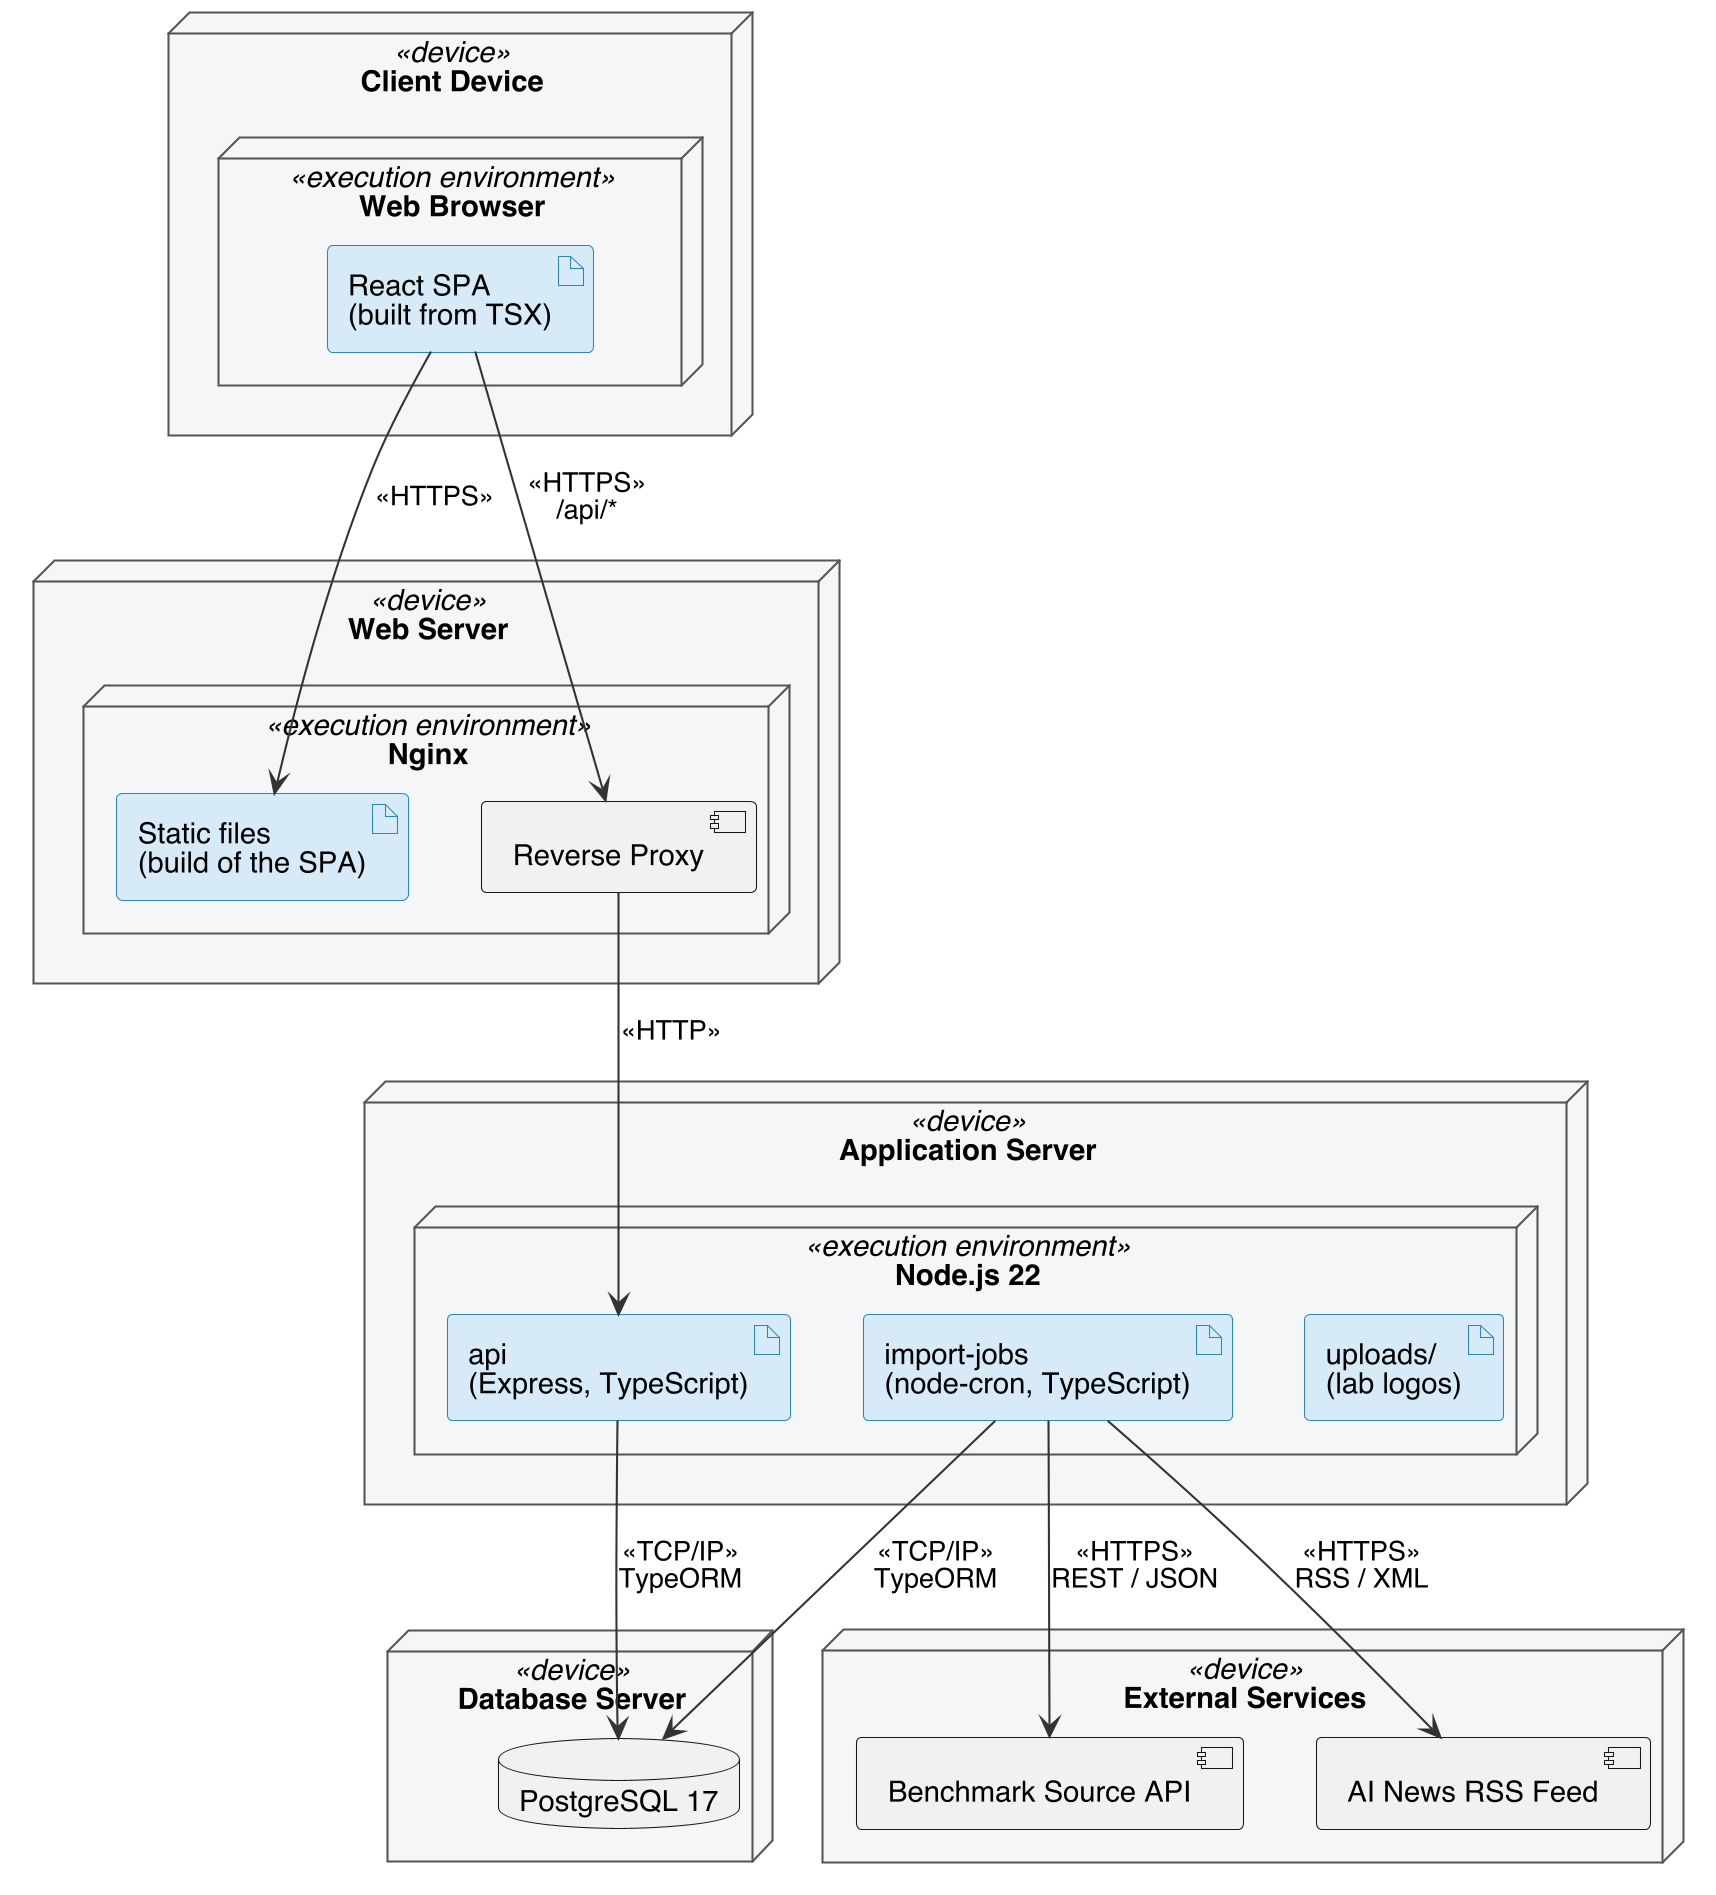
\includegraphics[width=\textwidth,height=0.7\textheight,keepaspectratio]{figures/deployment.png}
  \caption{Deployment diagram}
\end{figure}

\begin{itemize}
  \item \textbf{Client device:} the React SPA runs in the web browser of the user (computer or phone).
  \item \textbf{Web server:} Nginx serves the static files of the SPA and forwards the \texttt{/api/*} requests to the application server. HTTPS is enabled with a Let's Encrypt certificate.
  \item \textbf{Application server:} Node.js 22 runs the Express API and the import jobs. The TypeScript code is compiled with \texttt{tsc} before deployment. The lab logos uploaded by the administrator are saved in an \texttt{uploads/} folder on this server and served at \texttt{/uploads/*}; \texttt{labs.logo\_url} contains their path.
  \item \textbf{Database server:} PostgreSQL 17, saved every day.
  \item \textbf{External services:} benchmark source API and AI news RSS feed, called only by the import jobs.
\end{itemize}

For the course, the web server, the application server and the database can run on the same machine with Docker Compose (one container for each).

\section{Data Design}

The data model is written as TypeScript classes with TypeORM decorators (\texttt{@Entity}, \texttt{@Column}, \texttt{@ManyToOne}, \texttt{@OneToMany}\dots): each entity follows a class of the class diagram. TypeORM migrations create the PostgreSQL tables from these entities, and repositories give typed methods to read and write the data. The team never writes SQL by hand.


\textbf{Main tables:}
\begin{itemize}
  \item \texttt{users}(id, email, username, password\_hash, role, status, created\_at)
  \item \texttt{labs}(id, name, logo\_url)
  \item \texttt{models}(id, lab\_id, name, slug, release\_date, community\_score, community\_rank, benchmark\_score, benchmark\_rank)
  \item \texttt{model\_aliases}(id, source\_id, external\_name, model\_id)
  \item \texttt{votes}(user\_id, model\_id, type, updated\_at)
  \item \texttt{comments}(id, user\_id, model\_id, content, created\_at)
  \item \texttt{benchmarks}(id, name, description)
  \item \texttt{scores}(model\_id, benchmark\_id, source\_id, value, fetched\_at)
  \item \texttt{sources}(id, name, url, type, last\_success\_at, last\_error)
  \item \texttt{news}(id, source\_id, title, url, published\_at)
\end{itemize}

\begin{figure}[H]
  \centering
  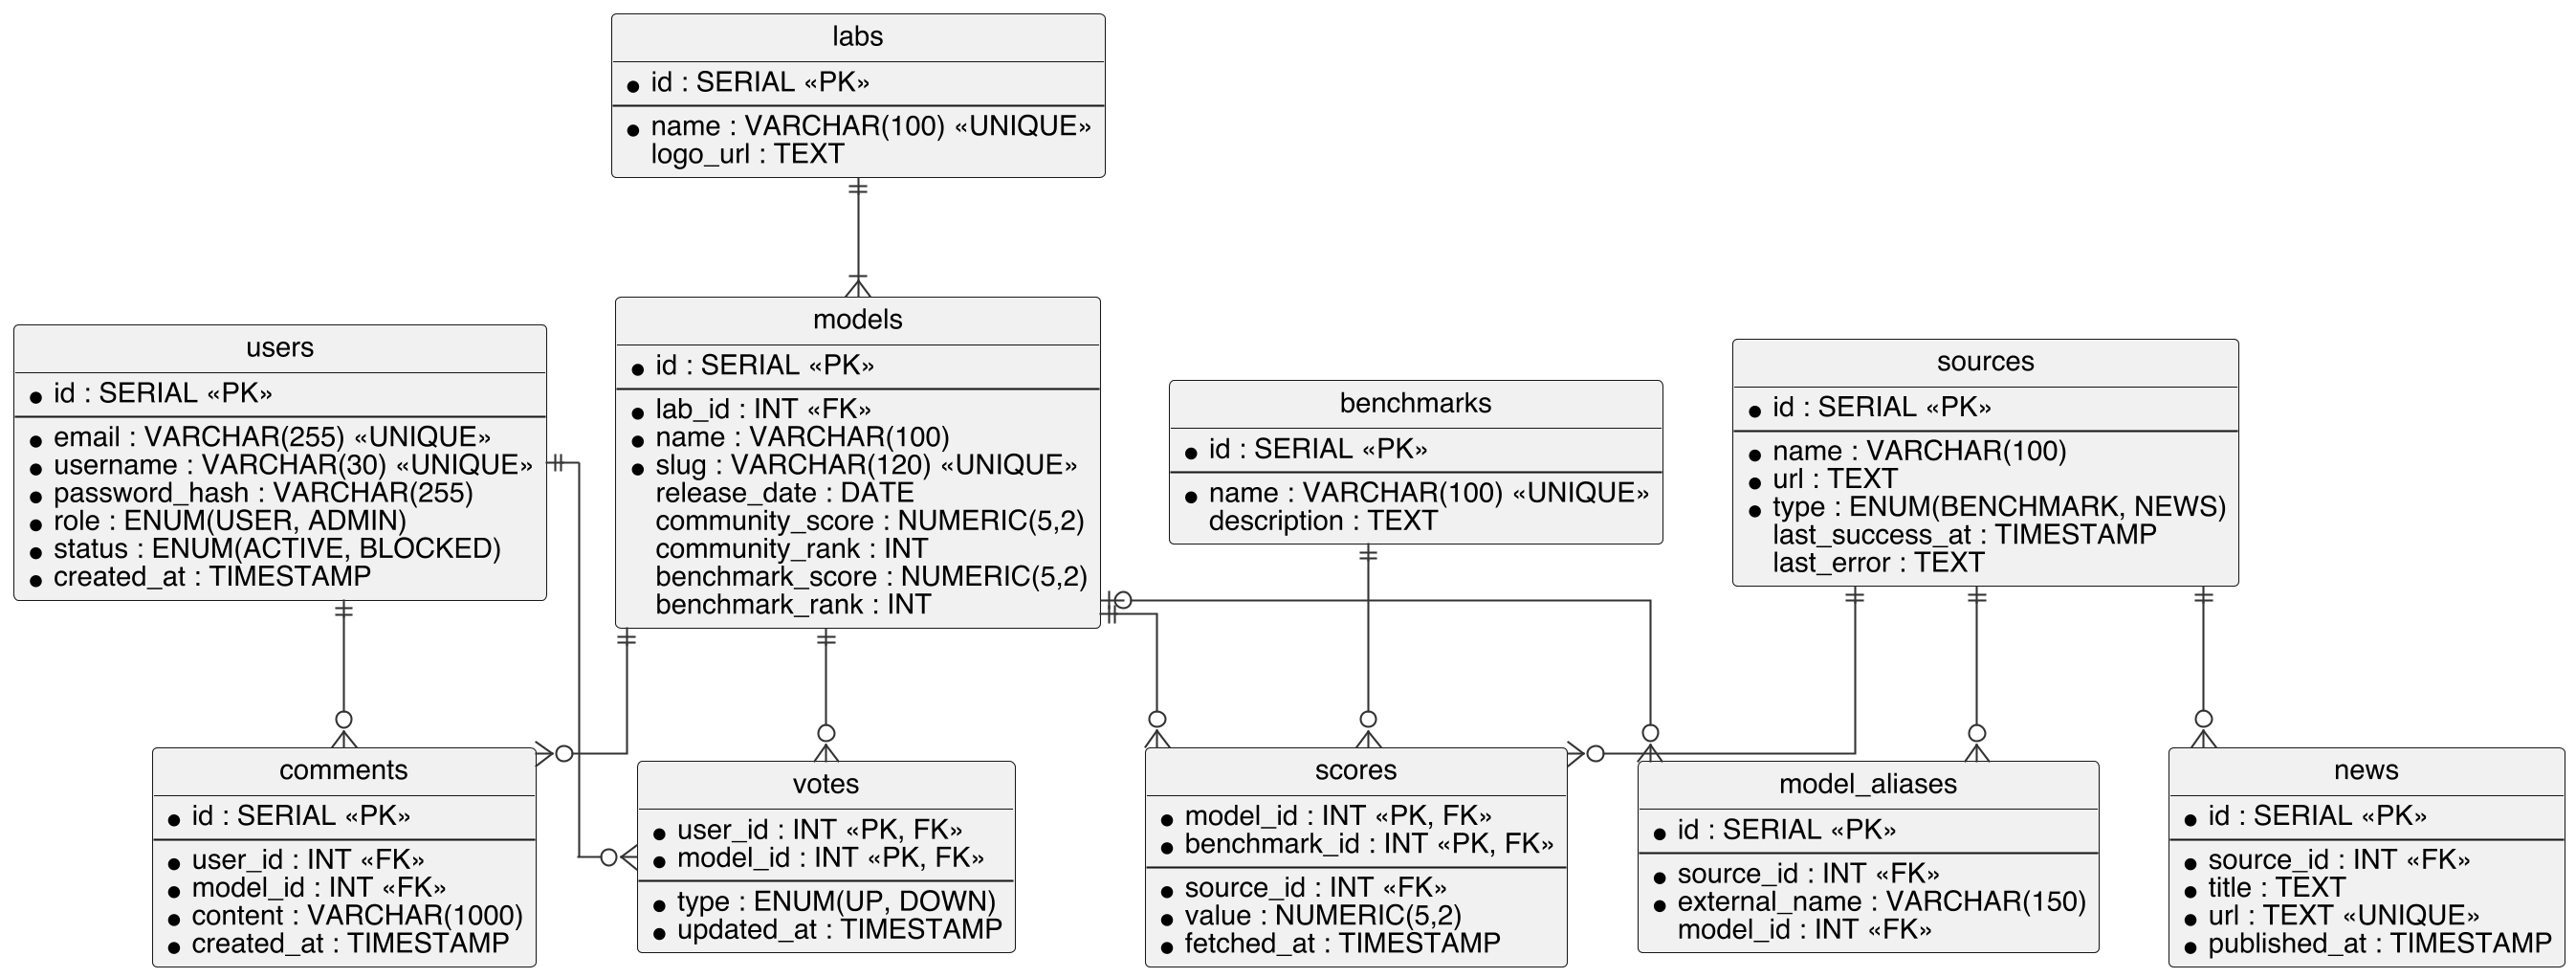
\includegraphics[width=\textwidth,height=0.7\textheight,keepaspectratio]{figures/er.png}
  \caption{Entity-relationship diagram}
\end{figure}

\textbf{Integrity rules:}
\begin{itemize}
  \item The primary key of \texttt{votes} is (\texttt{user\_id}, \texttt{model\_id}): a user can only have one vote per model.
  \item The primary key of \texttt{scores} is (\texttt{model\_id}, \texttt{benchmark\_id}): a model has only one score per benchmark.
  \item \texttt{votes.type} is \texttt{UP} or \texttt{DOWN}; \texttt{users.role} is \texttt{USER} or \texttt{ADMIN}; \texttt{users.status} is \texttt{ACTIVE} or \texttt{BLOCKED} (TypeORM enum columns).
  \item \texttt{scores.value} is between 0 and 100.
  \item The pair (\texttt{source\_id}, \texttt{external\_name}) of \texttt{model\_aliases} is unique. \texttt{model\_id} is empty while the name is not linked to a model.
  \item The score columns of \texttt{models} are empty only when the model has no vote (community) or no benchmark score (benchmark). The rank columns are empty when the model is not ranked (less than 10 votes or less than 3 benchmark scores). These columns are only written by RankingService.
  \item If two sources give the same benchmark for the same model, the most recent import replaces the old score; \texttt{scores.source\_id} always shows where the kept value comes from.
  \item \texttt{email}, \texttt{username} and \texttt{models.slug} are unique.
  \item When a user is deleted, their votes and comments are deleted too (TypeORM relation with \texttt{onDelete: 'CASCADE'}).
  \item A lab or a model cannot be deleted if it still has models, votes, comments or scores (TypeORM relation with \texttt{onDelete: 'RESTRICT'}).
\end{itemize}

\section{Interface Design}

\subsection{REST API}

All routes start with \texttt{/api}, use JSON, and return standard HTTP codes.

\begin{center}
\small
\begin{tabularx}{\textwidth}{llXl}
  \toprule
  \textbf{Method} & \textbf{Route} & \textbf{Description} & \textbf{Access} \\
  \midrule
  POST & \texttt{/auth/register} & Create an account & Public \\
  POST & \texttt{/auth/login} & Log in, set the session cookie & Public \\
  POST & \texttt{/auth/logout} & Log out & User \\
  GET & \texttt{/auth/me} & Current user & User \\
  DELETE & \texttt{/users/me} & Delete my account & User \\
  GET & \texttt{/labs} & Labs with their models & Public \\
  GET & \texttt{/models/\{slug\}} & Model details, scores, ranks, votes & Public \\
  GET & \texttt{/rankings?type=community|benchmark} & Ranking & Public \\
  POST & \texttt{/models/\{slug\}/vote} & Add, change or remove my vote & User \\
  GET & \texttt{/models/\{slug\}/comments} & Comments, newest first & Public \\
  POST & \texttt{/models/\{slug\}/comments} & Add a comment & User \\
  DELETE & \texttt{/comments/\{id\}} & Delete a comment (own, or any for admin) & User \\
  GET & \texttt{/news} & AI news, newest first & Public \\
  GET & \texttt{/admin/users} & List of users & Admin \\
  PATCH & \texttt{/admin/users/\{id\}} & Block or unblock a user & Admin \\
  DELETE & \texttt{/admin/users/\{id\}} & Delete a user & Admin \\
  GET & \texttt{/admin/comments} & Recent comments & Admin \\
  GET & \texttt{/admin/sources} & Import status of each source & Admin \\
  GET & \texttt{/admin/aliases} & Model names not linked yet & Admin \\
  PATCH & \texttt{/admin/aliases/\{id\}} & Link a name to a model, or create the model & Admin \\
  POST & \texttt{/admin/labs} & Create a lab (name + logo file) & Admin \\
  PUT & \texttt{/admin/labs/\{id\}/logo} & Replace the logo of a lab & Admin \\
  \bottomrule
\end{tabularx}
\end{center}

\textbf{Example:} \texttt{POST /api/models/gpt-5/vote} with \texttt{\{"type": "UP"\}} returns \texttt{200} with \texttt{\{"score": 82.4, "voteCount": 1204, "myVote": "UP"\}}.

\subsection{User Interface}

\begin{itemize}
  \item \textbf{Public pages:} home, models, model page, ranking, news, login.
  \item \textbf{User pages:} account page; vote and comment forms on the model page.
  \item \textbf{Admin page:} users, recent comments, import status, model names to link, lab logos. There is no link to this page: the administrator types \texttt{/admin}. The React route checks the role with \texttt{GET /api/auth/me}, and every admin API route checks it again on the server.
  \item \textbf{Menu:} Models, Ranking, News, and ``Log in'' for a guest, or ``Account'' and ``Log out'' for a logged-in user.
\end{itemize}

The wireframes are in the SRS (Section 6.1). The interface is built with Tailwind CSS and is responsive (mobile first).

\section{Detailed Design}

\subsection{Component Responsibilities}

\begin{itemize}
  \item \textbf{VoteService}
  \begin{itemize}
    \item Finds the existing vote of the user for the model.
    \item No vote: creates it. Same type: deletes it. Other type: updates it.
    \item Asks RankingService for the new community score.
  \end{itemize}
  \item \textbf{RankingService}
  \begin{itemize}
    \item Community score $=$ up / (up $+$ down) $\times$ 100, as soon as the model has one vote. The model gets a community rank only with at least 10 votes.
    \item Benchmark score $=$ average of the scores, as soon as the model has one score. The model gets a benchmark rank only with at least 3 scores.
    \item Sorts the models by score; in case of equality, the model with more votes (or scores) comes first.
    \item Saves the scores and ranks of all models in the \texttt{models} table, in one transaction. It runs after each vote (community ranking) and after each benchmark import (benchmark ranking). Pages only read these values, they never compute them.
  \end{itemize}
  \item \textbf{ImportService}
  \begin{itemize}
    \item One importer for each source, with the same interface: \texttt{fetch()}, \texttt{validate()}, \texttt{save()}.
    \item Validates the data with Zod before saving it.
    \item Saves everything in one transaction: if something fails, nothing is changed.
    \item News import: every 6 hours, reads the RSS feed of each NEWS source, and only saves the articles with a new URL (the URL is unique in \texttt{news}).
    \item Never creates a model automatically. Each external name is looked up in \texttt{model\_aliases}. If the name is unknown, it is saved as an unlinked alias and its score is ignored, until an administrator links it to an existing model or creates the model (with its lab).
  \end{itemize}
  \item \textbf{AuthService}
  \begin{itemize}
    \item Hashes the passwords with bcrypt.
    \item Creates a JWT stored in an HttpOnly cookie (valid 7 days). The token only contains the user id.
    \item Refuses the login if the account is \texttt{BLOCKED}.
    \item On every protected request, an Express middleware reads the user in the database and checks the status and the role. A blocked or deleted user gets a \texttt{403} (or \texttt{401}) and the cookie is cleared, so a block works immediately, even if the token is still valid.
  \end{itemize}
\end{itemize}

\subsection{Sequence -- Benchmark Import}

\begin{enumerate}
  \item Every day at 3:00, the Scheduler starts the benchmark import (the news import runs every 6 hours in the same way, without the ranking step).
  \item For each benchmark source, ImportService calls the external API.
  \item If the data is valid, ImportService saves all the scores in one transaction. Each external model name is matched with the \texttt{model\_aliases} table; unknown names are saved for the administrator and their scores are skipped.
  \item If there is an error, the old scores are kept and the error is saved in the \texttt{sources} table.
  \item At the end, RankingService computes the benchmark ranking again and saves it in the \texttt{models} table.
\end{enumerate}

\begin{figure}[H]
  \centering
  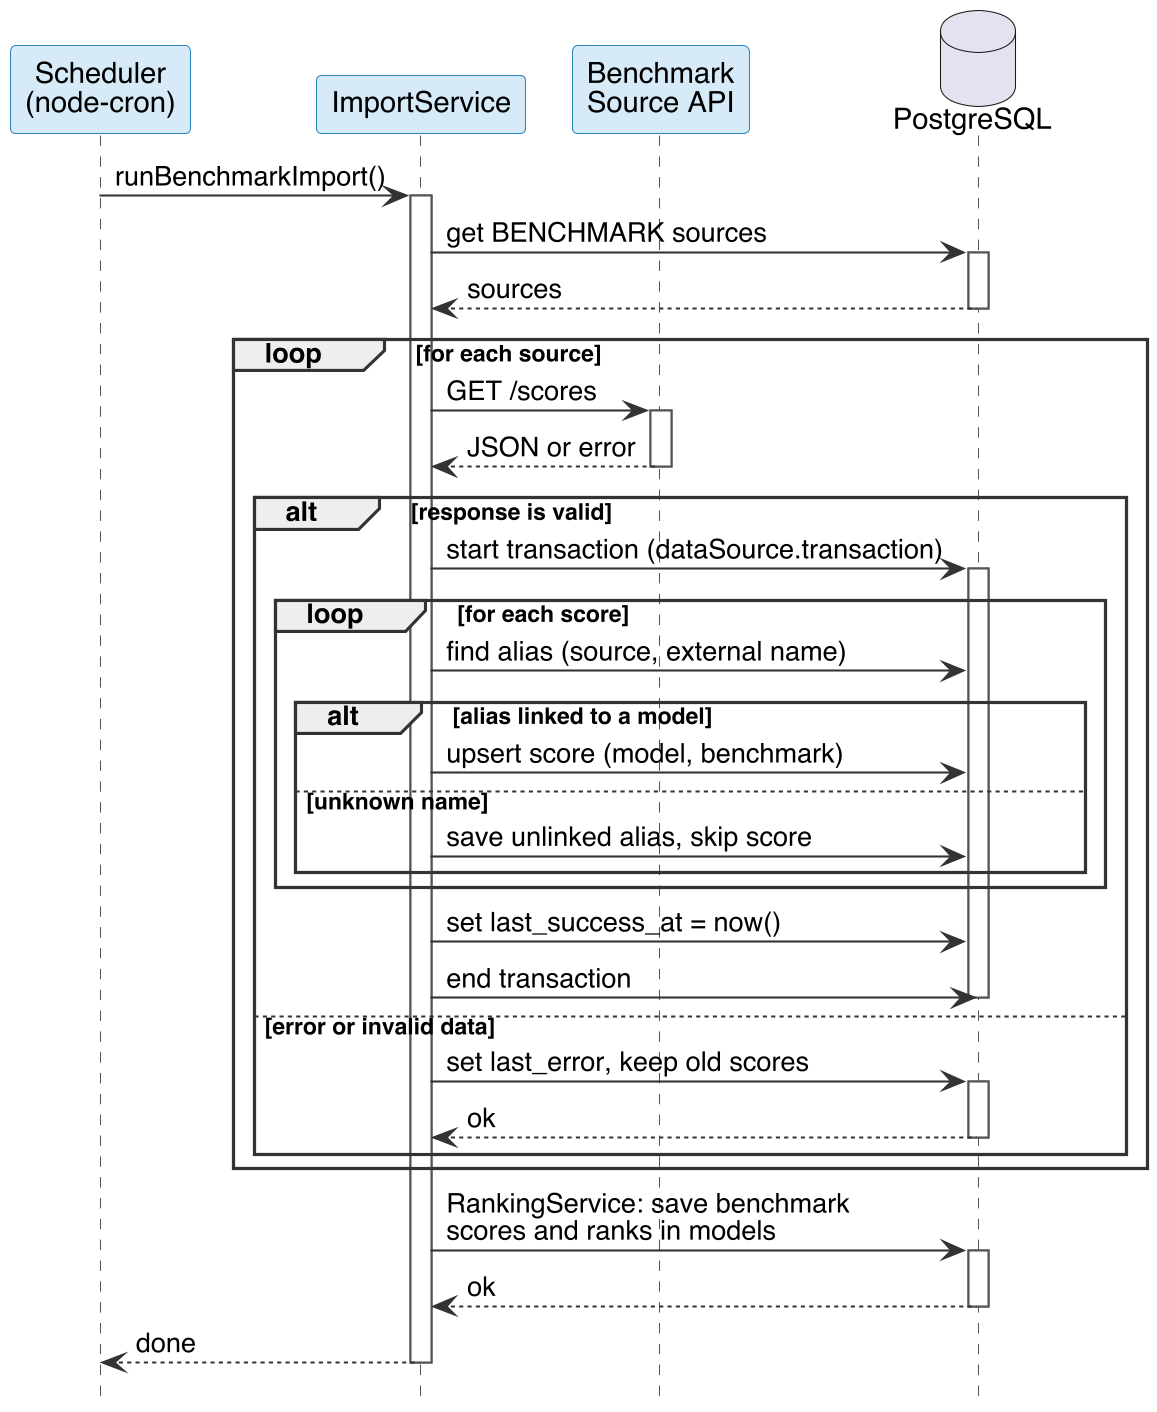
\includegraphics[width=\textwidth,height=0.65\textheight,keepaspectratio]{figures/import-sequence.png}
  \caption{Sequence diagram -- Benchmark import}
\end{figure}

\subsection{State Machine -- User Account}

After sign up, the account is \texttt{ACTIVE} and the user is logged in directly. Inside this state, the user is logged in or logged out; after an unblock, the user starts logged out. An administrator can block the account: the next request of the user is refused (the status is checked on every request) and the user cannot log in anymore. The account can be unblocked, or deleted.

\begin{figure}[H]
  \centering
  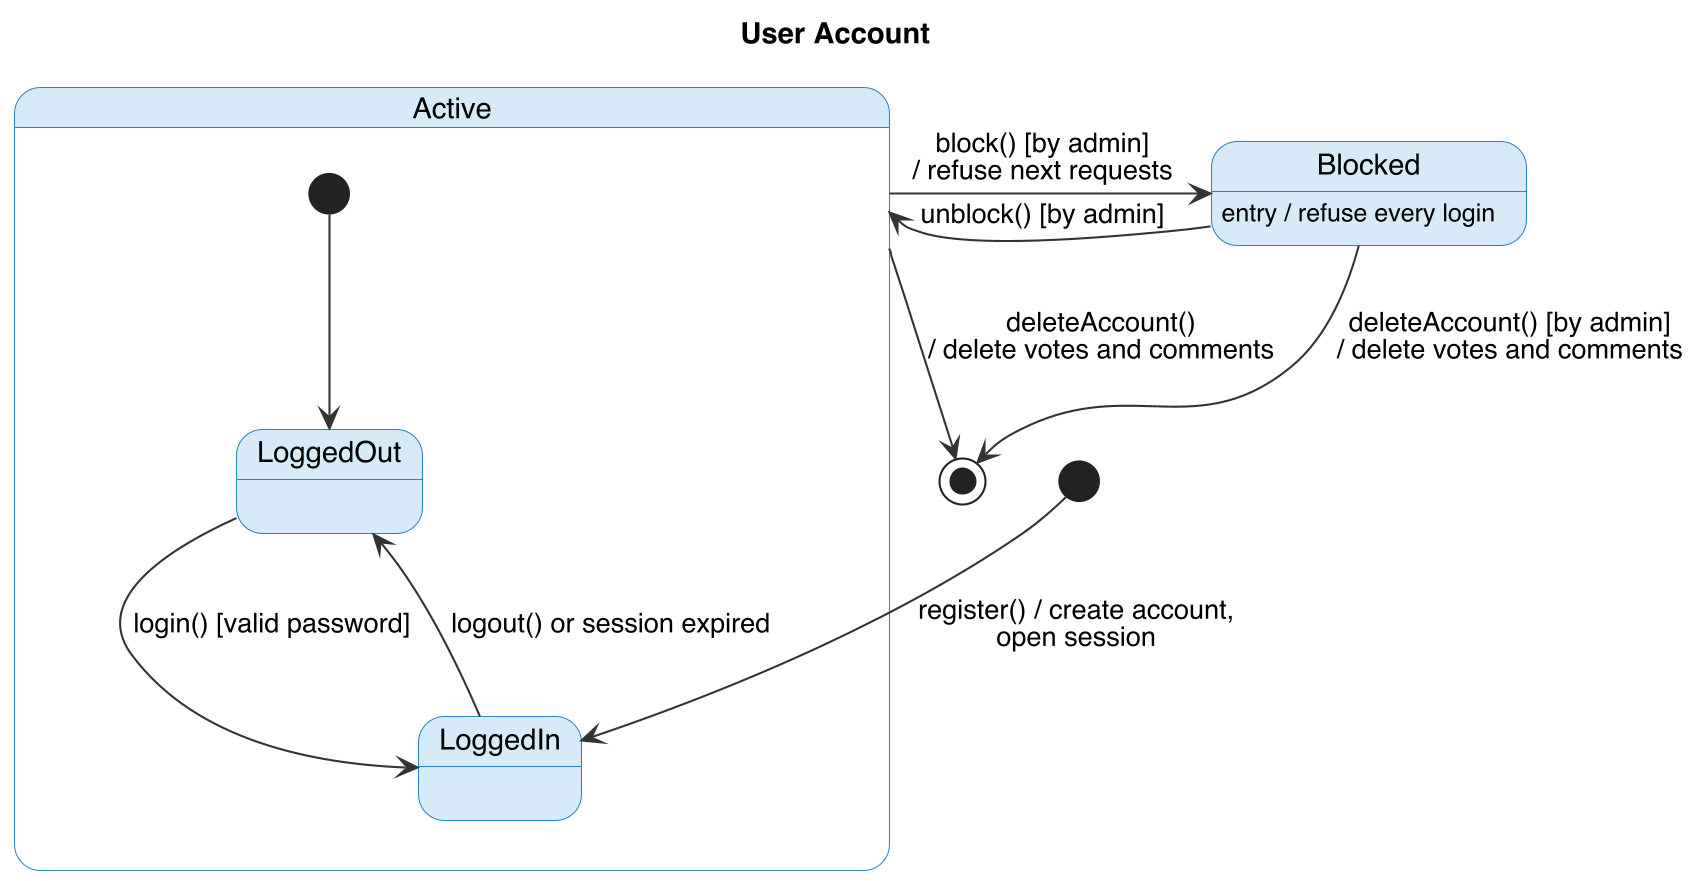
\includegraphics[width=0.85\textwidth,height=0.6\textheight,keepaspectratio]{figures/account-state.png}
  \caption{State machine diagram -- User account}
\end{figure}

\subsection{Error Handling and Recovery}

\begin{itemize}
  \item \textbf{400} for invalid data (for example an empty comment), with a clear message.
  \item \textbf{401} if the user is not logged in, \textbf{403} if the user does not have the right role or is blocked.
  \item \textbf{404} if the model, the comment or the user does not exist.
  \item \textbf{409} if the email or the username is already used.
  \item \textbf{500} for unexpected errors: a global Express error handler returns a generic message and logs the details.
  \item Import errors never stop the website: the last valid data is kept.
\end{itemize}

\section{Security and Compliance}

\begin{itemize}
  \item Passwords hashed with bcrypt; JWT in an HttpOnly, Secure, SameSite cookie.
  \item Role-based access control (visitor, user, admin) checked on every route by an Express middleware.
  \item HTTPS everywhere; security headers with Helmet; CORS limited to our frontend.
  \item Input validation with Zod; no SQL injection because all database access goes through TypeORM, which uses parameterised queries.
  \item Comments are displayed as plain text by React, which protects against XSS.
  \item Rate limiting on login and sign up to limit brute-force attacks and fake accounts.
  \item Logo upload (multer): only PNG, JPEG or WebP, 1\,MB maximum, file renamed with a random name. SVG is refused because it can contain scripts.
  \item The \texttt{/admin} page is not linked anywhere, but this is not the protection: the protection is the role check on the server.
  \item \textbf{GDPR:} only email, username and hashed password are stored; consent at sign up; account deletion removes all personal data, votes and comments.
\end{itemize}

\section{Performance, Scalability, Availability}

\begin{itemize}
  \item Scores and ranks are computed after each import or vote and stored in the \texttt{models} table, so a page view is only a simple read.
  \item Database indexes on \texttt{models.slug}, \texttt{votes.model\_id}, \texttt{comments.model\_id} and \texttt{scores.model\_id}.
  \item Comments are loaded by pages of 20.
  \item The API keeps no session in memory (JWT + database check), so more Node.js instances can be added behind Nginx if needed.
  \item Target: less than 2 seconds for each page with 100 users at the same time.
\end{itemize}

\section{Observability}

\begin{itemize}
  \item JSON logs for each request (method, route, status, duration) with the library Pino.
  \item Each import saves its result in the \texttt{sources} table (last success, last error), visible on the admin page.
  \item A \texttt{GET /api/health} route checks that the API and the database work.
\end{itemize}

\section{Internationalization and Accessibility}

\begin{itemize}
  \item The interface is in English at the start. All the texts are in one file, so another language can be added later.
  \item Dates are displayed in the format of the browser.
  \item Accessibility: labels on all form fields, keyboard navigation, good color contrast, and information never given only by color (for example, the selected vote arrow also changes its shape).
\end{itemize}

\section{Design Rationale}

\begin{itemize}
  \item \textbf{React + Node.js/Express in TypeScript:} React and Node.js are required by the course. TypeScript (strict mode, TSX for React) is used everywhere: the same language on both sides, and types shared between the frontend and the backend. No plain JavaScript files.
  \item \textbf{PostgreSQL:} relational data with strong constraints (one vote per user and model, cascade delete), which is important for our rules.
  \item \textbf{TypeORM:} ORM recommended in the course. It hides the SQL behind TypeScript classes and repositories, creates the migrations, and protects against SQL injection. Its entity classes are very close to our UML class diagram.
  \item \textbf{Imports saved in our database:} the website is faster and still works when an external source is down.
  \item \textbf{One service per feature:} the team can work in parallel, and a change in one feature does not break the others.
\end{itemize}

\section{Assumptions and Constraints}

\begin{itemize}
  \item Web application only; no native mobile app.
  \item The external sources are free and allow programmatic access.
  \item Team of four students, with the time of the course sprints.
  \item Hosting on one small server (or on the computers of the team for the demo).
\end{itemize}

\section{Open Issues and Future Work}

\begin{itemize}
  \item Final choice of the benchmark source and of the news feed.
  \item Suggestions for the administrator when linking model names (today, the link is fully manual).
  \item Detection of fake accounts and vote manipulation.
  \item Replies to comments and reports of bad comments by the users.
  \item History of the rankings over time.
\end{itemize}

\end{document}
